\subsection{Sorting Algorithms}
    \subsubsection{Selection Sort}
        \begin{minipage}{0.59\linewidth}
            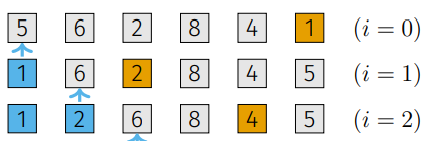
\includegraphics[width = \linewidth]{src/6_algorithms/images/selection_sort.png}
        \end{minipage}
        \begin{minipage}{0.39\linewidth}
            \fcolorbox{black}{cyan}{sorted list}\\
            \fcolorbox{black}{white}{unsorted list}\\
            \fcolorbox{black}{orange}{smallest value}
        \end{minipage}

        \lstinputlisting{src/6_algorithms/code/4_selection_sort.py}
        
        \begin{tabular*}{\linewidth}{| p{0.25\linewidth} | p{0.35\linewidth} | p{0.22\linewidth} |}
            \hline
            Case & Description & Runtime\\
            \hline \hline
            Worst-case & A is reverse sorted & $\Theta(n^2)$ \\
            \hline
            Average-case & - & $\Theta(n^2)$ \\
            \hline
            Best-case & A is already sorted & $\Theta(n)$ \\
            \hline
        \end{tabular*}
        
    \subsubsection{Insertion Sort}
        \begin{tabular*}{\linewidth}{| p{0.25\linewidth} | p{0.35\linewidth} | p{0.22\linewidth} |}
            \hline
            Case & Description & Runtime\\
            \hline \hline
            Worst-case &  &  \\
            \hline
            Average-case &  &  \\
            \hline
            Best-case &  &  \\
            \hline
        \end{tabular*}

    \subsubsection{Bubble Sort}
        
    \subsubsection{Mergesort (Divide and Conquer)}
        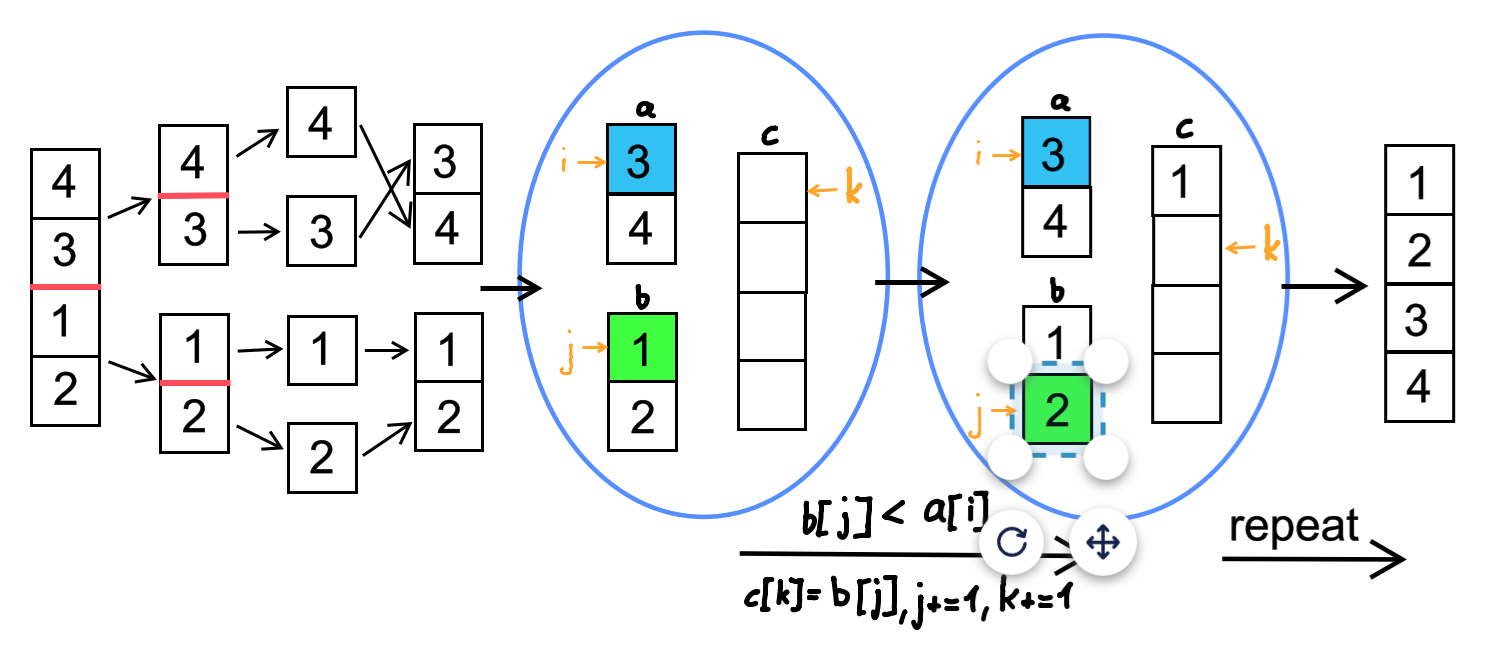
\includegraphics[width = \linewidth]{src/6_algorithms/images/mergesort.png}
        \fcolorbox{black}{cyan}{greater value}  \fcolorbox{black}{green}{smaller value}

        \lstinputlisting{src/6_algorithms/code/4_mergesort.py}

        \begin{tabular*}{\linewidth}{| p{0.25\linewidth} | p{0.35\linewidth} | p{0.22\linewidth} |}
            \hline
            Case & Description & Runtime\\
            \hline \hline
            All cases & - & $\Theta (n \cdot \log(n))$ \\
            \hline
        \end{tabular*}
    
    \subsubsection{Quick Sort (Divide and Conquer)}
        